\chapter{Conceptual framework}

This chapter describes the conceptual framework of the method used by \dfastmi and the derivation of the river parameters used for the Dutch rivers.

\section{Characteristics of bed level changes due to river measures}

A river measure, i.e.~a local river adjustment (typically a flow capacity enlarging adjustment) outside the main channel, may result in changes in the flow pattern within the main channel.
The bed levels within the main channel will react to such changes depending on the

\hspace{1cm}\emph{magnitude, duration and length scale of these flow pattern changes in the main channel.}

Hence, the core focus of the rule-of-thumb is to determine and characterize the changes in the flow pattern within the main channel.
Here, we define the main channel as the part of the river between the groyne heads.

At the upstream end of the floodplain adjustment part of the main channel discharge will leave the main channel, which will flow through the enlarged floodplain, secondary channel or bank area, and return to the main channel at the downstream end of the project area.
The resulting changes in the main channel flow pattern cause sedimentation in the main channel at the upstream "offtake" of the new outflow and erosion at the downstream "confluence" when the flow enters the main channel again.
Because the river discharge varies, the pattern will also vary during the year
As a result a part of the main channel bed level adjustment is stationary and a part of the adjustment is transitional and it will migrate downstream.
A reduction in the water depth may thus not only be observed locally where the flow diverges into the flood plain, but also downstream thereof.

The bed level change due to river enlargement can largely be characterized as follows

\begin{itemize}
\item The magnitude of the bed level change varies over the seasons; the maximum change is observed at the end of the flood season and the adjustment reaches a minimum at the end of the low flow period.

\item Local evaluation of the bed level changes is insufficient because of partial downstream migration of the bed level changes.

\item The maximum impact is observed on that side of the river which is closest to the adjustment.
\end{itemize}

Because part of the bed level changes migrate downstream, the morphological impact on projects located downstream may be increased.
After all, the maximum bed level change of one single river enlarging measure is reached at the end of the flood period and it's the result of that flood period.
However, when a series of measures along the river are combined (for instance, lowering of the groynes along a reach) the downstream bed level changes may be increased by accumulation of downstream migrating bed waves, such that the accumulated bed level change may be significantly larger.
In other words, river measures extending over longer reaches may result in a larger morphodynamic response than comparable but more isolated measures.

The aforementioned observations result in the following premises.
The rule-of-thumb described in the following sections

\begin{itemize}
\item will only be valid for the estimation of the impact of local measures with a length of at most one flood plain,

\item should take into account seasonal variations, and

\item needs to be estimate the spatial pattern of the bed level change.
\end{itemize}


\section{Characterization of the changes in the main channel flow pattern}

When a measure in the floodplains does not include something like a permanently active secondary channel, the flow pattern in the main channel will only be affected during flood conditions.
If on the other hand, such a secondary channel (or other measure active under medium to low flow conditions such as groyne adjustments) is included in the design then the flow pattern will also be influenced during transitional or even low flow conditions.
It's therefore critical to determine the effect of the measure on the main channel flow pattern at different discharge levels.

Secondary channels may have a major impact on the morphodynamics of the main channel.
The magnitude of the discharge through the secondary channel varies as function of the river discharge.
Because the hydraulic conditions of the secondary channel can change over time (e.g.~due to vegetation, siltation, or erosion) the discharge through a secondary channel is typically controlled by some hydraulic structure.
The typical characteristics of a weir (Dutch: overlaat, drempel) and orifice (Dutch: onderlaat, duiker) are shown in \autoref{Fig1}.

\begin{figure}[b]
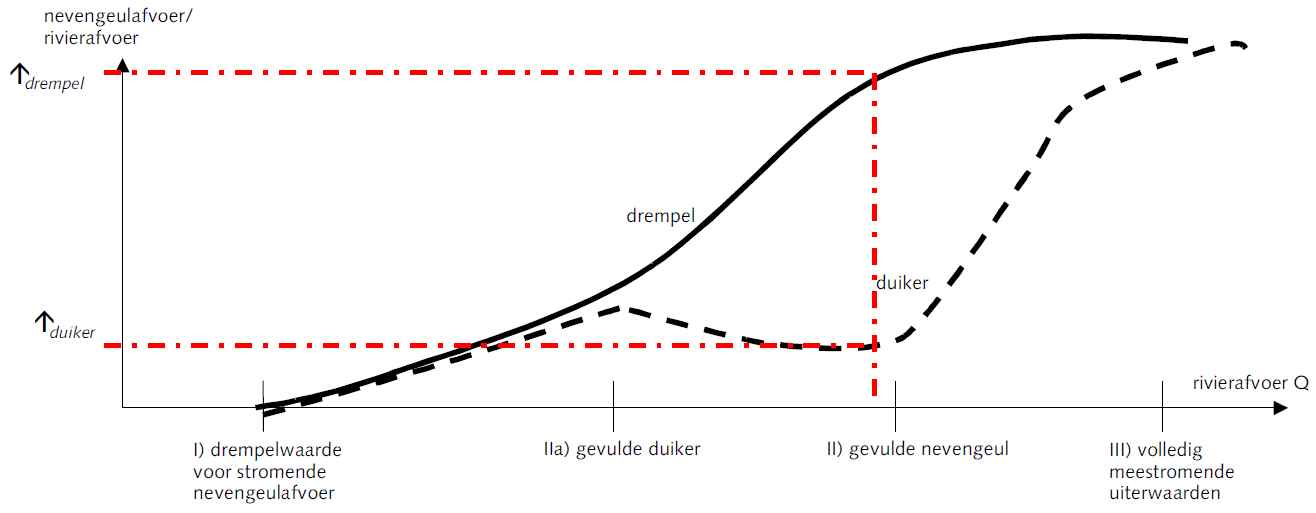
\includegraphics[width=\columnwidth]{figures/Fig1.png}
\caption{Schematic of the controlled discharge through a secondary channel.}
\label{Fig1}
\end{figure}

The discharge through a secondary channel is characterized by a number of special conditions as illustrated by \autoref{Fig1}:

\begin{enumerate}
\item the beginning of flow through the secondary channel
\item the bankfull secondary channel
\item the fully developed flow in the secondary channel and surrounding floodplain.
\end{enumerate}

When the discharge through the secondary channel is controlled by an orifice, the fully flooded condition may add an additional characteristic discharge.
In order to characterize the flow patterns during flood it's necessary to distinguish the condition in which the flood plains just start to carry flows, and the condition of fully developed flow in the flood plains.
\dfastmi version 2 and before (in WAQMORF) used an algorithm to determine which three flow conditions would best represent the effect of the measure under various conditions.
However, as these conditions varied depending on the thresholds specified by the user, the tool could give different results depending on the user.
In \dfastmi version 3, a new method has been implemented that removes most input parameters; only the minimum discharge at which the measure becomes active is still used as an input besides the general location characteristics of the branch and reach in which the measure is located.

\section{Scientific background}
\todo{Scientific background to be included.}
A general introduction on the use of a ``hydrograph'' approach configured in the rivers configuration file: for the bovenrivieren a set of discharges, extended to a combination of discharge and tidal boundary conditions in the future for the benedenrivieren